This chapter is devoted to describing the outcomes of the preliminary research focusing on the similar already existing projects and technologies we could utilize.
In section \ref{txt:similar_projects} the similar projects will be described together with their relations to our project and their advantages and disadvantages. 
Then in the section \ref{txt:development technologies} the development technologies and colaboration tools will be presented with outcome of the overall research. 


\section{Similar projects} \label{txt:similar_projects}

We were not able to find any other service that would use exactly the same technical solution as compared to our product. 
Nevertheless a few similar entertainment services that aim to amuse the music concert audience already exist. 
These services basically encourage the audience to use either their smartphones or other device as the source of light that helps to create impressive and colorful show.

\subsection{Wham City Lights}

\subsubsection{Description}
The Wham City Lights is the mobile application developed by the one year old Baltimore based start-up \footnote{\url{http://whamcitylights.com/}}. 
As far as the Digital Lighter is concerned the Wham City Light service seems to be the closest solution as it works with the users' smartphones and uses them as a source of the light and even the sound.

Users attending the given concert only need to download and install the free application, start it and then hold their smartphones in the air.
The application then controls the color displayed on the smartphone screen, the camera flashes and the sound going out of the speakers and it creates the spatial soundscapes and lighting designs.
What is more the application do not require the Internet connection as the instructions are modulated into the ultrasonic inaudible signal that is being continuously transmitted during the performance.

Using this innovative technique all of the smartphones can be effectively synchronized so that the  changing lights and imagery on the phone follows and complete the music performance.
Nevertheless the so called light show must be pre-programmed and this system cannot determine the location of the mobile devices.

The demonstration of the real world performance of the application and the whole concept for that matter can be seen in the official Wham City Lights marketing video\footnote{\url{http://www.youtube.com/watch?v=faJ1Av5kBCE}}.

\begin{figure}[!t]
	\centering
		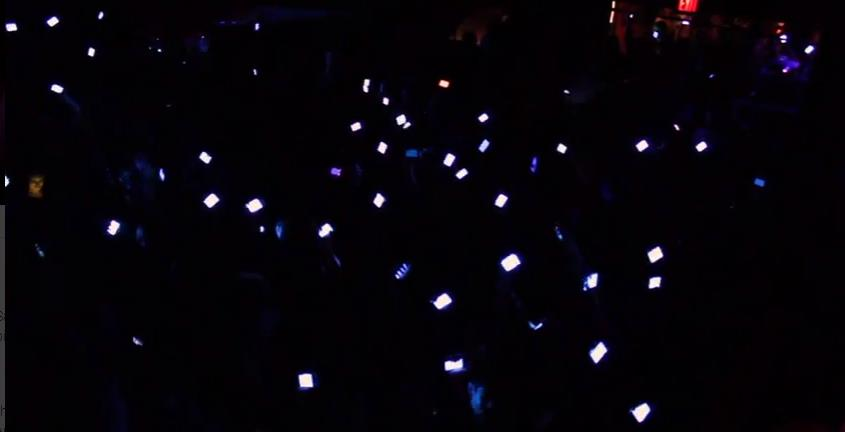
\includegraphics[width=10cm]{preliminaryStudies/wham_city_lights.jpg}
	\caption{Wham City Lights}
	\label{fig:wham_city_lights}
\end{figure}

\subsubsection{Impact}
The Wham City Lights application or its derivatives have been so far used on relatively many music events of the greater importance where several thousands of people were present and used the application. To list a few:
\begin{itemize}
\item America's Got Talent 2013
\item CMA Music Festival 2013
\item Intel sales conference 2013
\item Billboard Music Awards 2013
\item etc.
\end{itemize}

\subsubsection{Availability}
The application is available for the devices using Android or iOS operating systems and it can be downloaded from the Google Play\footnote{https://play.google.com/store/apps/details?id=com.whamcitylights} and App Store\footnote{https://itunes.apple.com/us/app/wham-city-lights/id580034697?mt=8} respectively. The developer nevertheless offers the customers the concert specific applications with relevant user interface built-in. As for the light show itself, programming part can be done either by the customer or the developer.

\subsubsection{Relation to our project}
Like our project the Wham City Lights application build upon users' smartphones that are remotely controlled in order to display intended imagery. 

\paragraph{Advantages}
The devices attending the light show do not need the Network connection and the displayed imagery is well synchronized with the music.

\paragraph{Disadvantages}
The location of the mobile devices cannot be determined and the different processing speed of the devices causes incorrect synchronization.


\subsection{Xylobands}

\subsubsection{Description}
So called Xyloband\footnote{http://xylobands.com/} is the invention of the company RB Concepts Limited. The device itself consists of the plastic bracelet that includes the LED diodes of the different colors and the microcontroller. 
The bracelets are controlled by the radio signal being broadcast from the stage and as a result they change their colors, flashes and in general create colorful imagery.

\begin{figure}[!t]
	\centering
		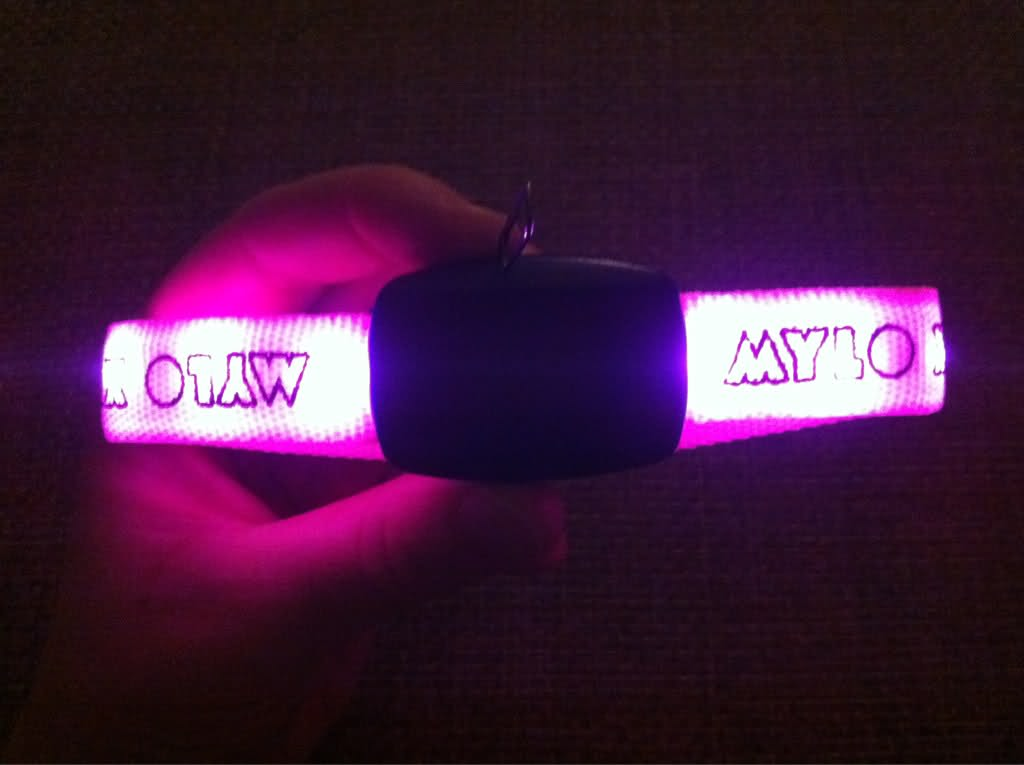
\includegraphics[width=10cm]{preliminaryStudies/xylo.jpg}
	\caption{Wham City Lights}
	\label{fig:xylo}
\end{figure}

\subsubsection{Impact}
Xylobands received great fame thanks to the well known British rock band ColdPlay which used them during their 2012 tour.

\subsubsection{Availability}
The bracelets can be ordered on the official Xylobands website.

\subsubsection{Relation to our project}
the Xylobands product is somewhat different from the Digital Lighter as it does not utilize the users' mobile devices. 
The similarity can be found in the way the bracelets are synchronized using wireless signal. 

\paragraph{Advantages}
The users do not need to bring their own mobile device and all of the audience have the possibility to become the part of the light show.

\paragraph{Disadvantages}
The location of the single participants cannot be determined.

%\section{Existing technologies and frameworks}
%\section{Evaluation of alternative solutions}

\section{Development technologies} \label{txt:development technologies}

According to the customer's requirements the product must be executable on the mobile devices and it should utilize the image processing technologies as well. Therefore we had to make two main decisions - which mobile platform to prefer and which existing image processing libraries to use. Both of the decisions are explained in greater detail in sections \ref{txt:mobile_platform} and \ref{txt:image_processing_library}.

\subsection{Mobile platform - Android} \label{txt:mobile_platform}

The mobile devices market is currently flooded with smartphones and tablets running on dozen of different platforms. 
But since we try to aim the application on as many users as possible the choice was relatively straightforward.
Considering the survey carried on by the well established analyst, the company IDC, as of Q2 2013 Google's Android OS held almost 80 \% of the market share\footnote{\url{http://www.idc.com/getdoc.jsp?containerId=prUS24257413}} leaving iOS, windows Phone, BlackBerry and others well behind.
What is more all of the members of our team posses the Android based smartphone thus we decided to choose the Android platform.

\subsubsection{Android SDK}

Google provides the Android developers with all the necessary tools and API's through the open source and free SDK\footnote{Software Development Kit}. While developing under SDK the Java programming language together with the Android event-driven architecture is used.

\subsubsection{Android NDK}

Through the NDK\footnote{Native Development Kit} Google provides the toolset allowing the programmers parts of the application using native-code languages such as C and C++.
We discussed using NDK just for the computationally demanding modules such as the image processing since the applications based on already compiled code tend to run faster.
Nevertheless we are allowed to scale the problem down and thus the use of Java perfectly suffices fr our purposes.
Should the customer require to scale the problem up we can switch to using NDK anytime.

\subsection{Image processing library - OpenCV} \label{txt:image_processing_library}

As far as the image processing is considered the outcome of our preliminary research is as follows.
Currently there exist a few open source and free libraries generally focusing on working with the multimedia.
OpenCV library is probably the most well-known library providing a broad range of image processing functions.
It is written and meant to be used in conjunction with C++ but the possibility to use Java already exists too.
The support for using OpenCV on Android platform is provided through the OpenCV4Android SDK that can be obtained from the official OpenCV website\footnote{\url{http://docs.opencv.org/}} and used for free.
So far we consider this toolkit to be sufficient for our needs but should we come across any problems we might be forced to switch to the combination of OpenCV, C++ and Android NDK.


\section{Development tools} \label{txt:development tools}

\subsection{Project management tool}
Since we use Scrum methodology, we were in need to find an appropriate management tool supporting Scrum. 
There exist many possible tools, but most of them are charged from
certain number of team members. 
Here are presented tools we have used for a testing purposes or in real development.

\paragraph{Trello}
is a collaboration tool\footnote{\url{https://trello.com/}} that can organize tasks into various boards, it shows what task has been assigned to who and in what stage the task is.
Even though Trello supports a lot of features, it is not originally designed for Scrum use and there is no support of \emph{Epics}, \emph{Burn-down chart} and time tracking.

\paragraph{Gravity} 
is a simple project management tool\footnote{\url{www.gravitydev.com}} currently in beta phase.
It supports splitting stories into tasks and also automatically calculates \emph{Burn-down chart}. 
Last but not least it supports it is free of charge for 5 team members, it supports issue tracking and support labels, which can be used for \emph{Epics}.
On the other hand it does not support time tracking.
You can see picture of Gravity's features in image \ref{img:gravity}.

\begin{figure}[!h]
	\centering
		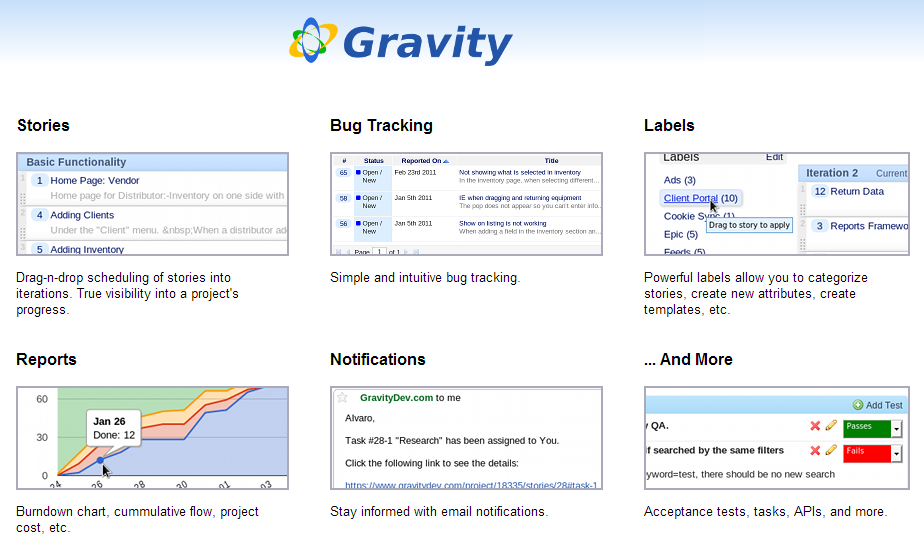
\includegraphics[width=11cm]{preliminaryStudies/gravity.png}
	\caption{Gravity features}
	\label{img:gravity}
\end{figure}

\paragraph{Target Process} is a project management tool\footnote{\url{http://www.targetprocess.com/}} that supports different processes such as Scrum, Kanban and own process. 
To its main features belongs role distinguishing, different graphs (such as \emph{Burn-down chart}), time estimation and time tracking of both stories and its tasks, drag and drop prioritizing which makes it easy to use from customer side and different kinds of boards (diverse point of views on project).
On the contrary it also does not support Epics and it is much more complicated to use than other tools introduced.
You can see example of board in TargetProcess3 in image \ref{img:targetp}.

\begin{figure}[!t]
	\centering
		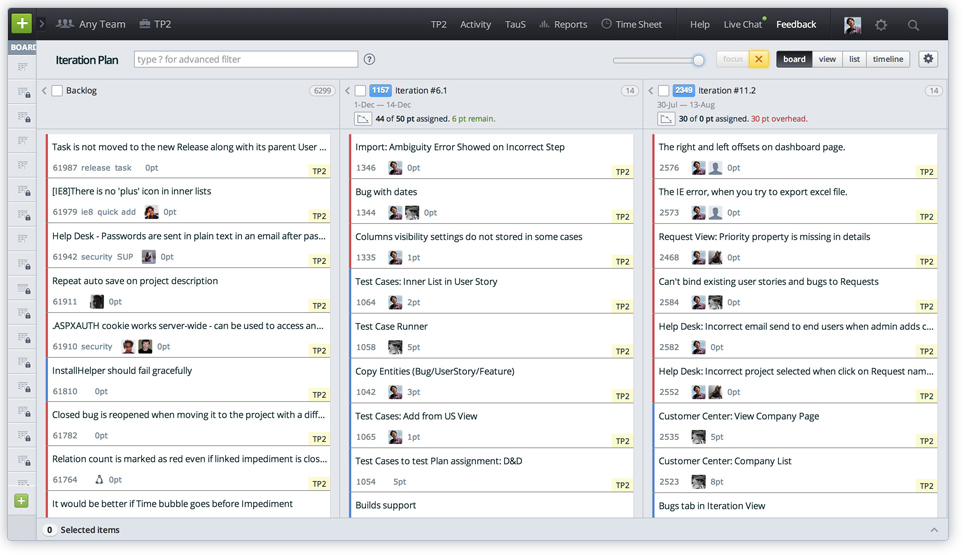
\includegraphics[width=11cm]{preliminaryStudies/targetp.png}
	\caption{TargetProcess's board}
	\label{img:targetp}
\end{figure}

\paragraph{Summary}
After short discussion we have decided that Trello is not suitable for our purpose so we started to use Gravity since 
we still did not know which features we will need since we were not skilled in Scrum methodology.
After a while it showed up, that Gravity has some bugs since it is in Beta version and also miss time tracking feature.
Because of that in 30th of August we have decided to start using TargetProcess3 although its complexity.


\subsection{Version control system}
Version control systems (VCS) are usually stand-alone applications but they can be integrated into other applications. These system usually allow users to browse previous versions of content.

We have decided that we will use VCS both for source code of applications and for project report. As every member of the team had experience with different version control systems, they become our candidates.
As our team works both on Microsoft Windows and GNU/Linux, it is necessary that chosen VCS supports clients in both platforms.
Another criteria was support of online code repository free of charge.

\paragraph{Subversion} or SVN is an open source centralized VCS and has many clients across different platforms. 
SVN is supported by Google Code\footnote{\url{http://code.google.com/}} repository.
SVN supports atomic commits, branching and more.

\paragraph{Git} on the other hand is distributed VCS and offers immediate offline operations.
Projects like Linux kernel\footnote{\url{https://www.kernel.org/}} and Glibc\footnote{\url{https://www.gnu.org/software/libc/}} are using Git as a VCS.
Although Git was created by Linus Torvalds, there are Windows clients available.
Git is supported by GitHub\footnote{\url{https://github.com/}}, what is web-based hosting service for VCS.

\paragraph{Summary} We have adopted Git as our version control system due to our customer suggestion, the distribution feature and our good experience with Github.
You can find our repository on \url{https://github.com/dohnto/CDP} page.


\begin{figure}[!t]
	\centering
		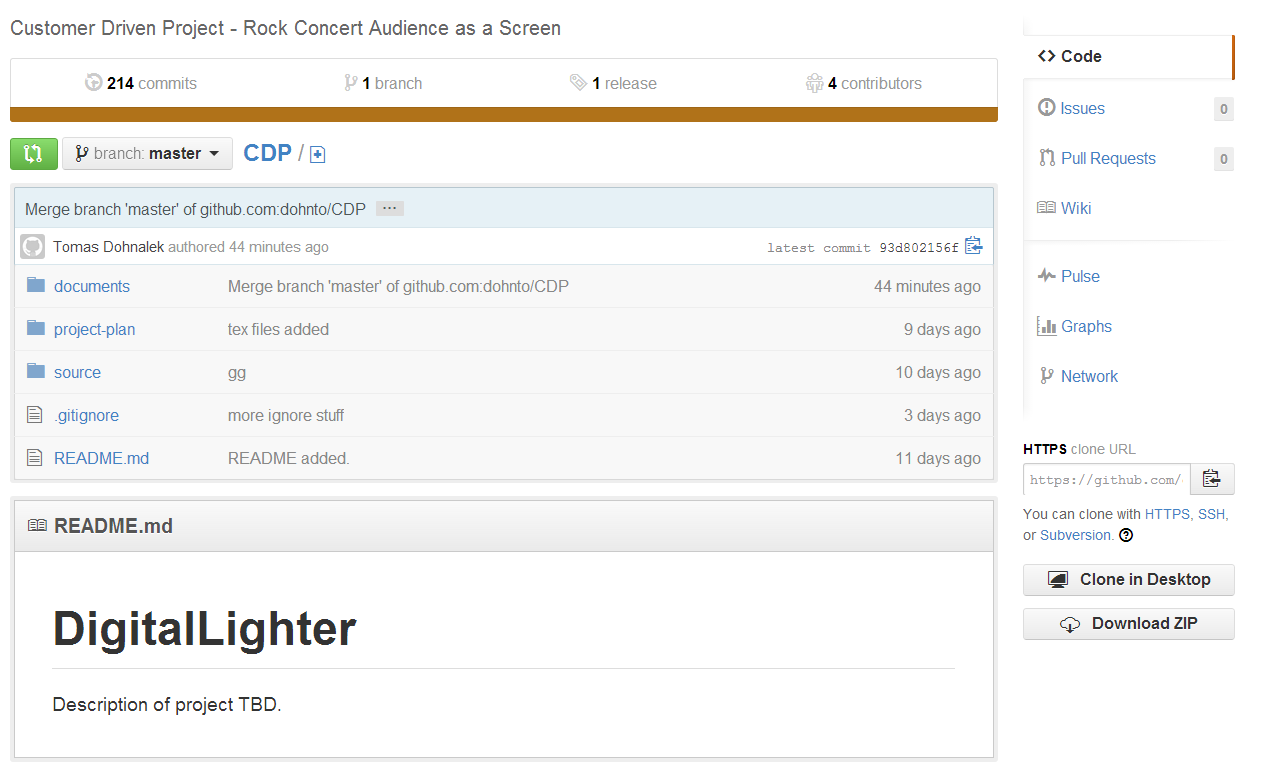
\includegraphics[width=10cm]{preliminaryStudies/git.png}
	\caption{Our github page}
	\label{img:git}
\end{figure}

\section{Outcome of research}
